\chapter{Multi view terrestrial laser scan registration (steps 2 and 3)}
\section{Step 2}
\begin{figure}[H]
	\centering
	\includegraphics[width=\textwidth]{10.png}
	\caption{Load session.json prepared by 'Lidar odometry'.}
	\label{fig:10}
\end{figure}

\begin{figure}[H]
	\centering
	\includegraphics[width=\textwidth]{13.png}
	\caption{Prepare field of view and change decimation to see more points. Generate random colors option is recommended for next steps as every scan will be in a different color.}
	\label{fig:13}
\end{figure}

\begin{figure}[H]
	\centering
	\includegraphics[width=\textwidth]{14.png}
	\caption{Turn on Manual Pose Graph Loop Closure Mod, then choose two different scans that share scanned objects, but difference in their numbers is as big as possible e.g. when you made a loop during scanning and came back to the same place after some time. Then click add edge.} 
	\label{fig:14}
\end{figure}

\begin{figure}[H]
	\centering
	\includegraphics[width=\textwidth]{15.png}
	\caption{Turn on manipulate active edge, turn on gizmo and align scan to scan manually.}
	\label{fig:15}
\end{figure}

\begin{figure}[H]
	\centering
	\includegraphics[width=\textwidth]{16.png}
	\caption{Once You are not capable align more accurate, then turn off gizmo and repetitively use ICP until scans align to the level at which nothing can change anymore.}
	\label{fig:16}
\end{figure}

\begin{figure}[H]
	\centering
	\includegraphics[width=\textwidth]{17.png}
	\caption{Turn off manipulate active edge, click "set initial poses as motion model", then click "compute pose graph SLAM".}
	\label{fig:17}
\end{figure}

\begin{figure}[H]
	\centering
	\includegraphics[width=\textwidth]{18.png}
	\caption{Turn off Manual Pose Graph Loop Closure Mod and inspect if everything is ok, if not,  repeat steps from figures 3.3-3.6 (choose another pair of scans, refine them and compute the pose graph SLAM).}
	\label{fig:18}
\end{figure}

\begin{figure}[H]
	\centering
	\includegraphics[width=\textwidth]{19.png}
	\caption{Once the job is done click Save session button to save changes to session.json and export data to *.laz. The latter is Your map that can be loaded by e.g. \href{https://www.cloudcompare.org/}{CloudCompare}.}
	\label{fig:19}
\end{figure}
\pagebreak
{\large \textbf{Should division of the session be needed, follow the steps below that describe how to do this using step 2 of the HDMapping program:}}
\begin{figure}[H]
	\centering
	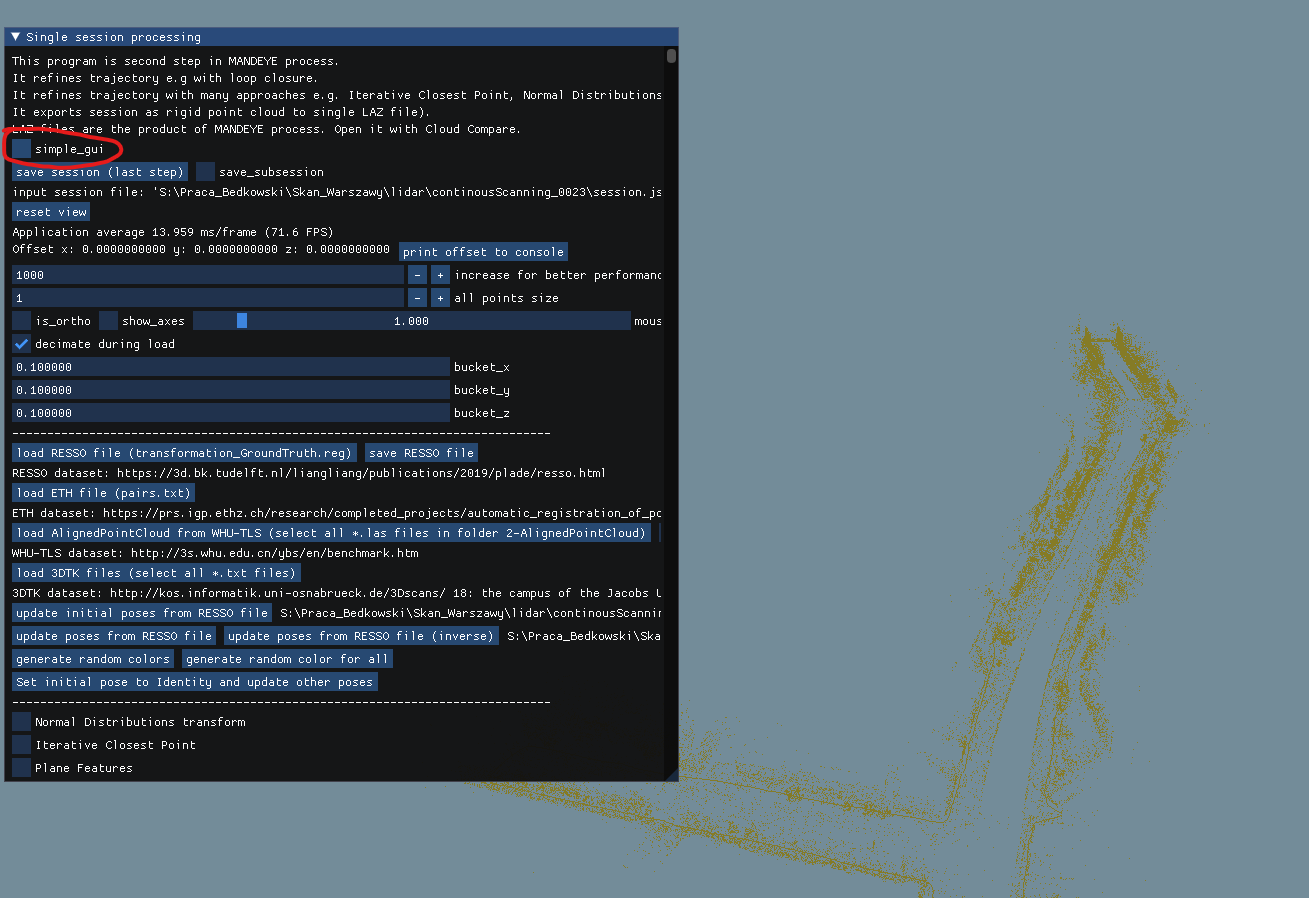
\includegraphics[width=\textwidth]{Cut_session1.png}
	\caption{Load the session as usual into step 2, prepare boundary scan numbers that will outline parts of scans, when prepared toggle off the simple gui.}
	\label{fig:20}
\end{figure}

\begin{figure}[H]
	\centering
	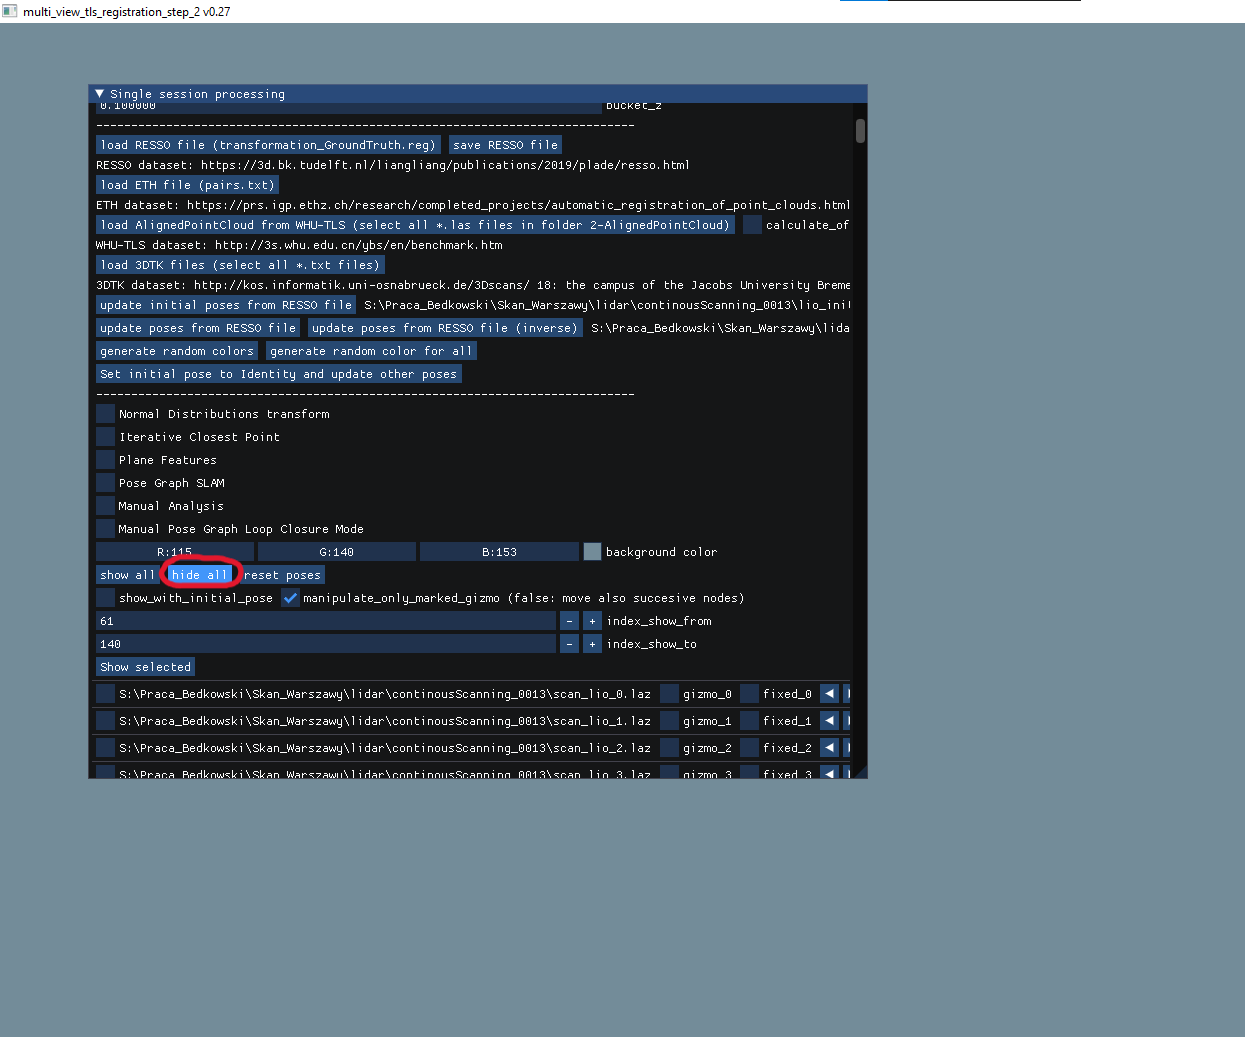
\includegraphics[width=\textwidth]{Cut_session2.png}
	\caption{Scroll down to list of scans and click hide all.}
	\label{fig:21}
\end{figure}

\begin{figure}[H]
	\centering
	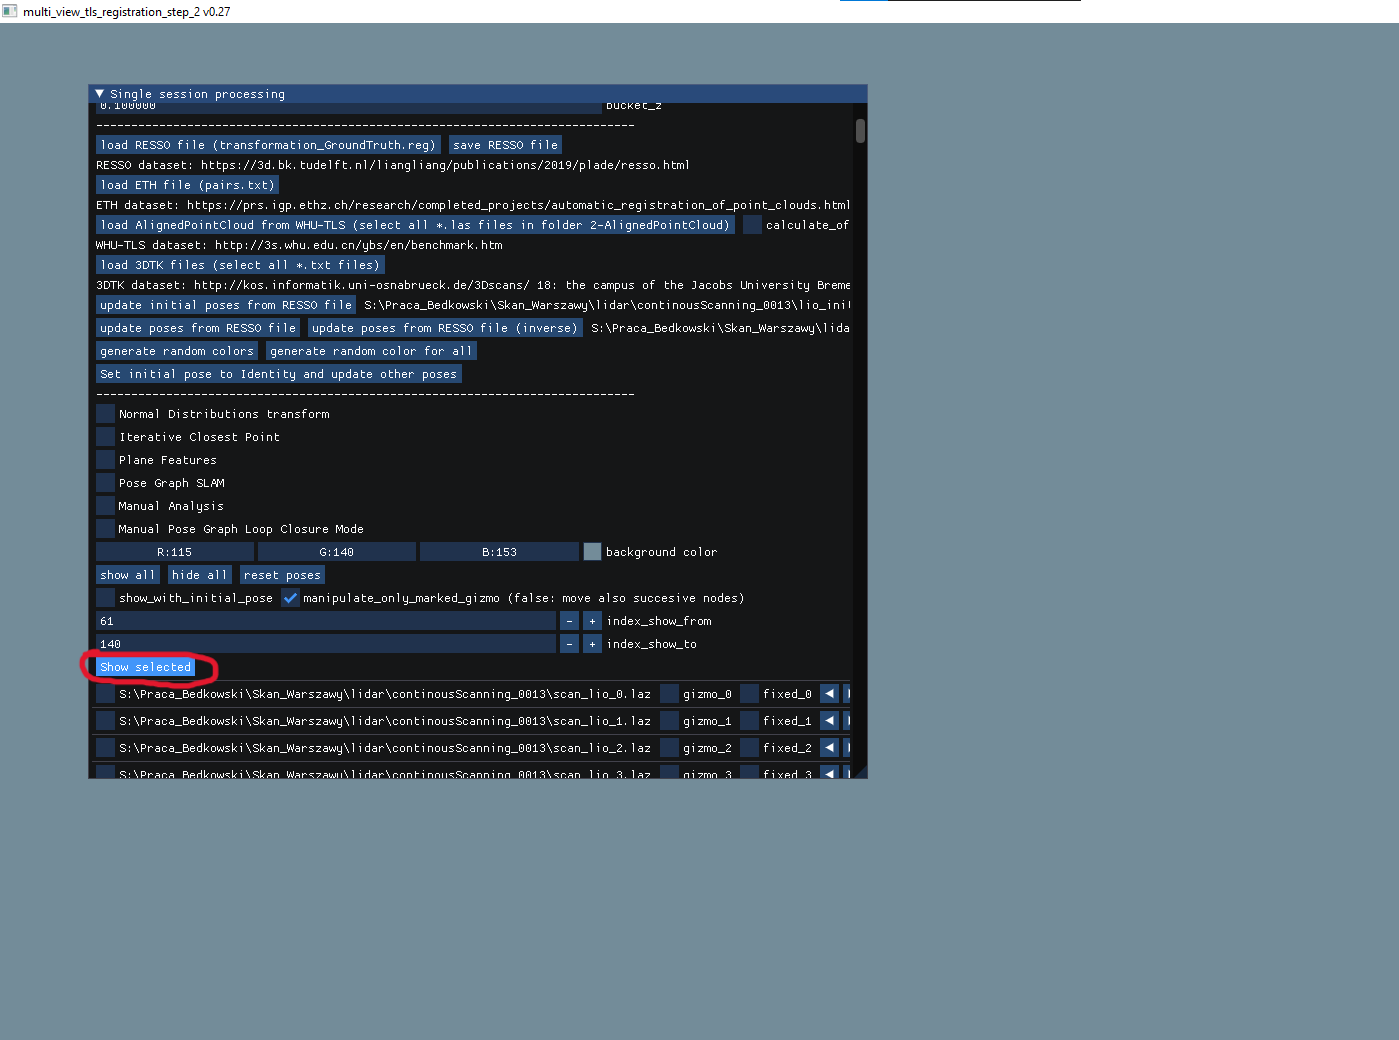
\includegraphics[width=\textwidth]{Cut_session3.png}
	\caption{Write indexes of the beginning scan and ending scan then click Show selected. The scans between the indicated ones will appear. This step may be repeated to build a session form many, separated fragments.}
	\label{fig:22}
\end{figure}

\begin{figure}[H]
	\centering
	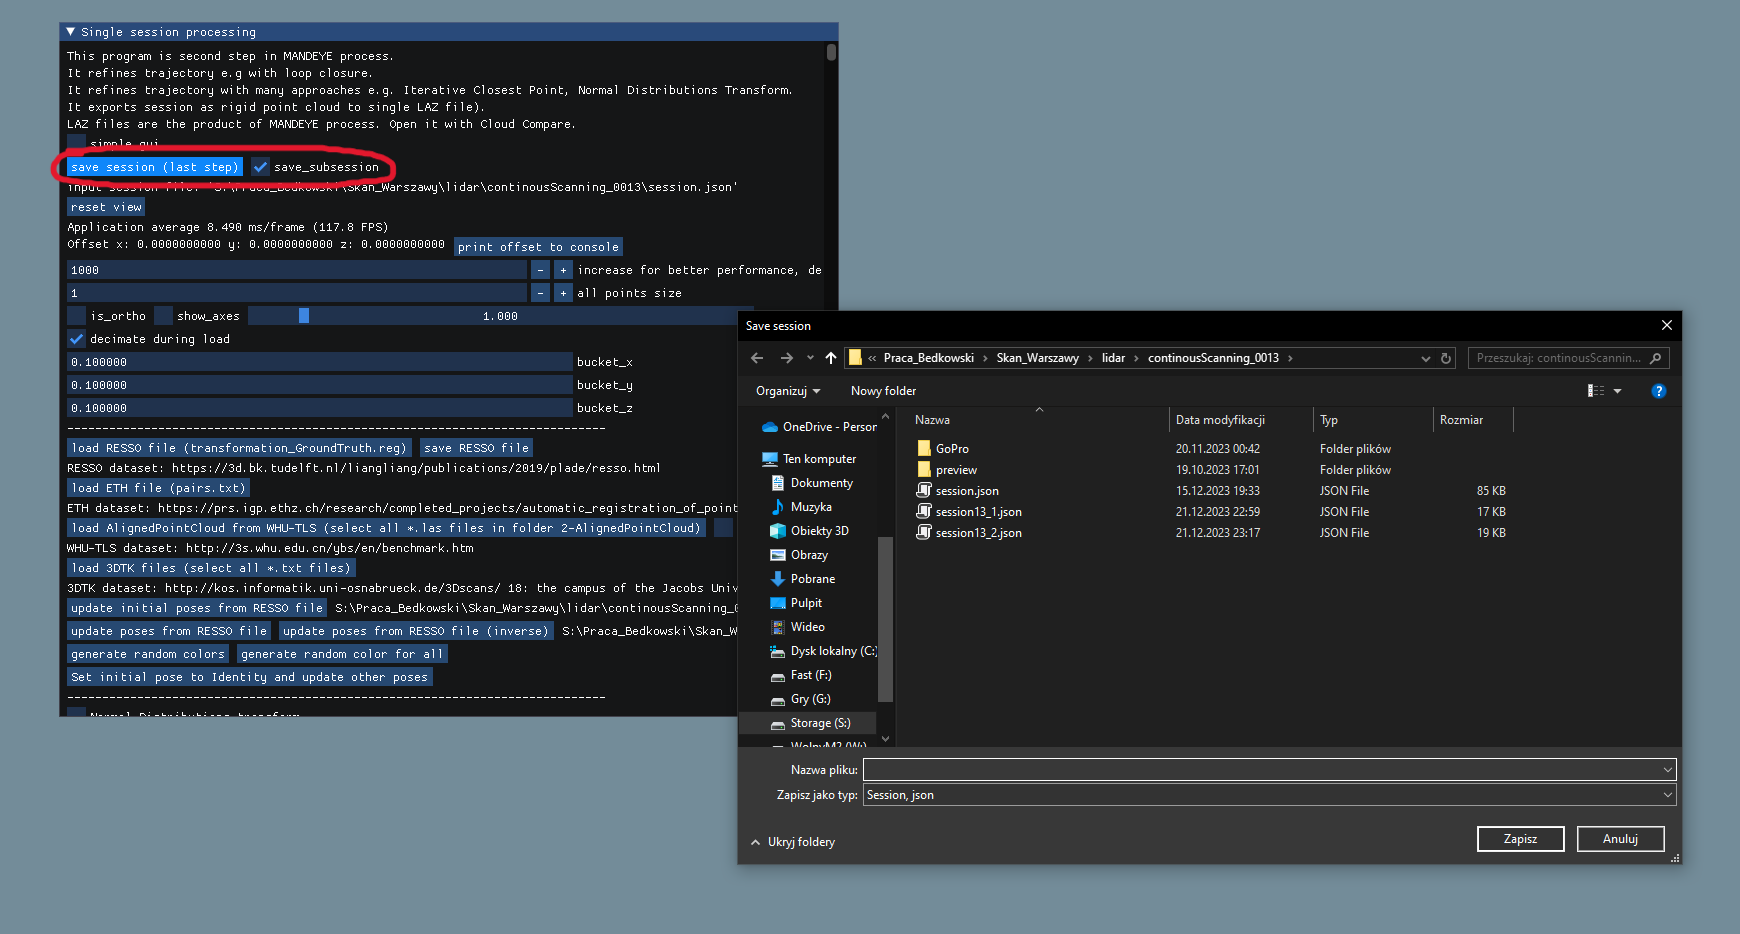
\includegraphics[width=\textwidth]{Cut_session4.png}
	\caption{With desired scans selected scroll up, select save subsession and click save session. Save the session to a new .json session file.}
	\label{fig:23}
\end{figure}

\begin{figure}[H]
	\centering
	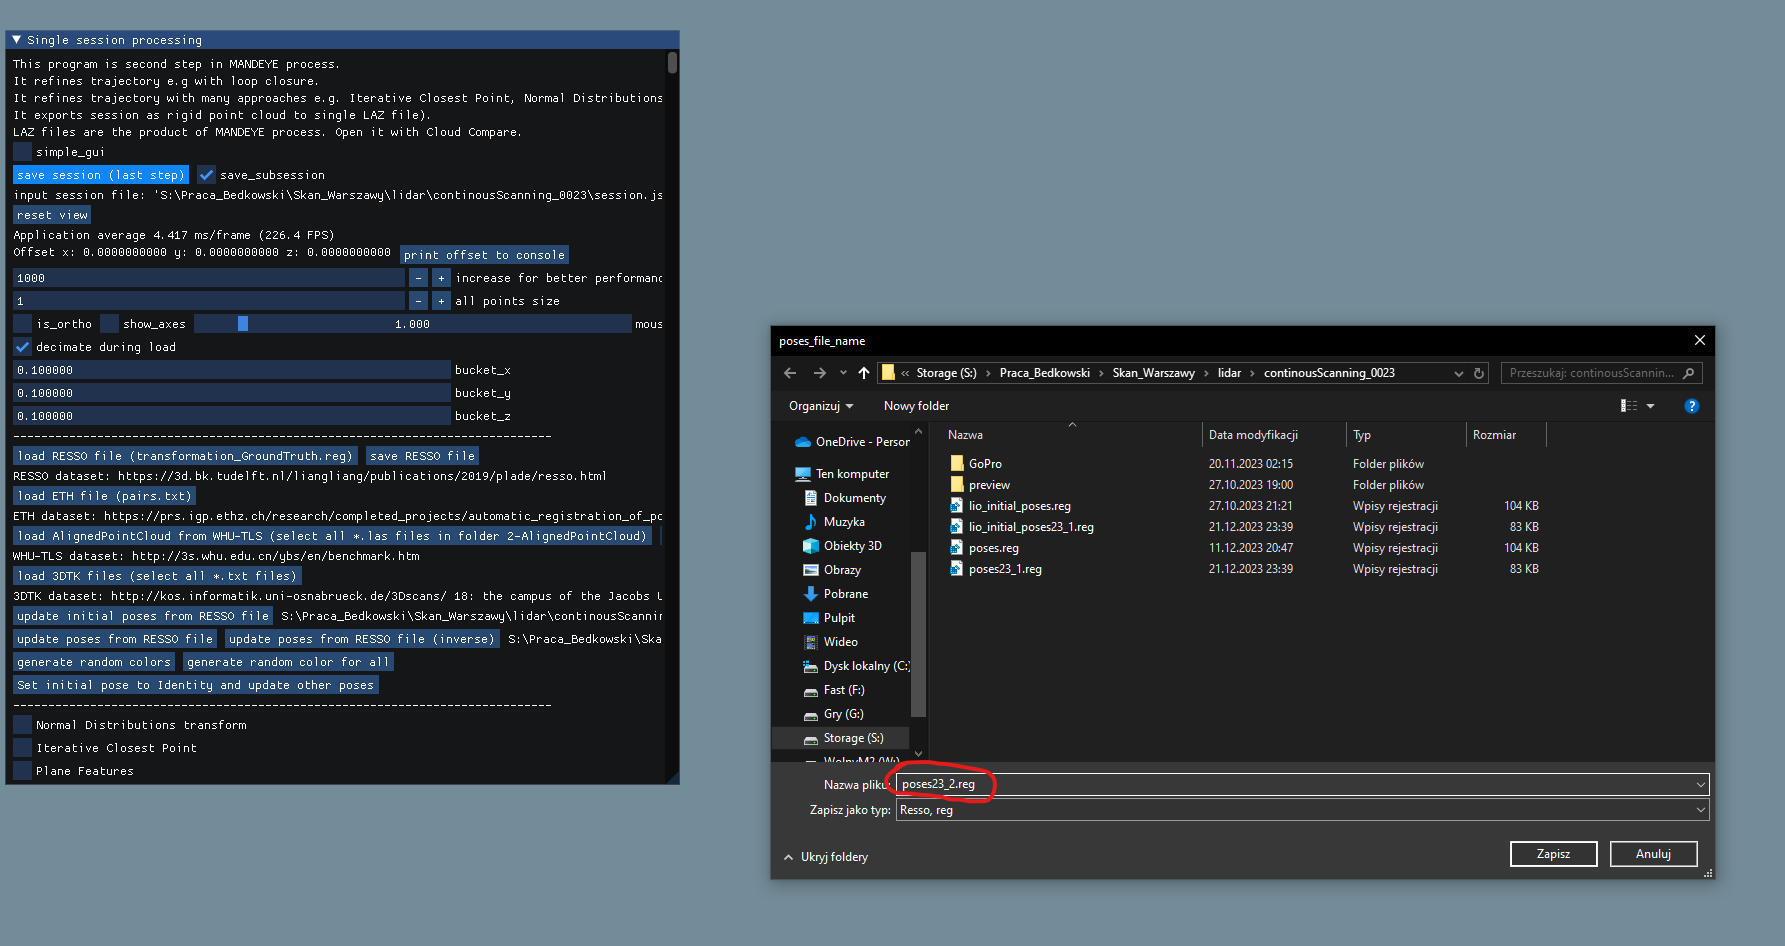
\includegraphics[width=\textwidth]{Cut_session5.png}
	\caption{After a .json session file is saved, proceed with creating new resso .reg file and saving poses to it.}
	\label{fig:24}
\end{figure}

\begin{figure}[H]
	\centering
	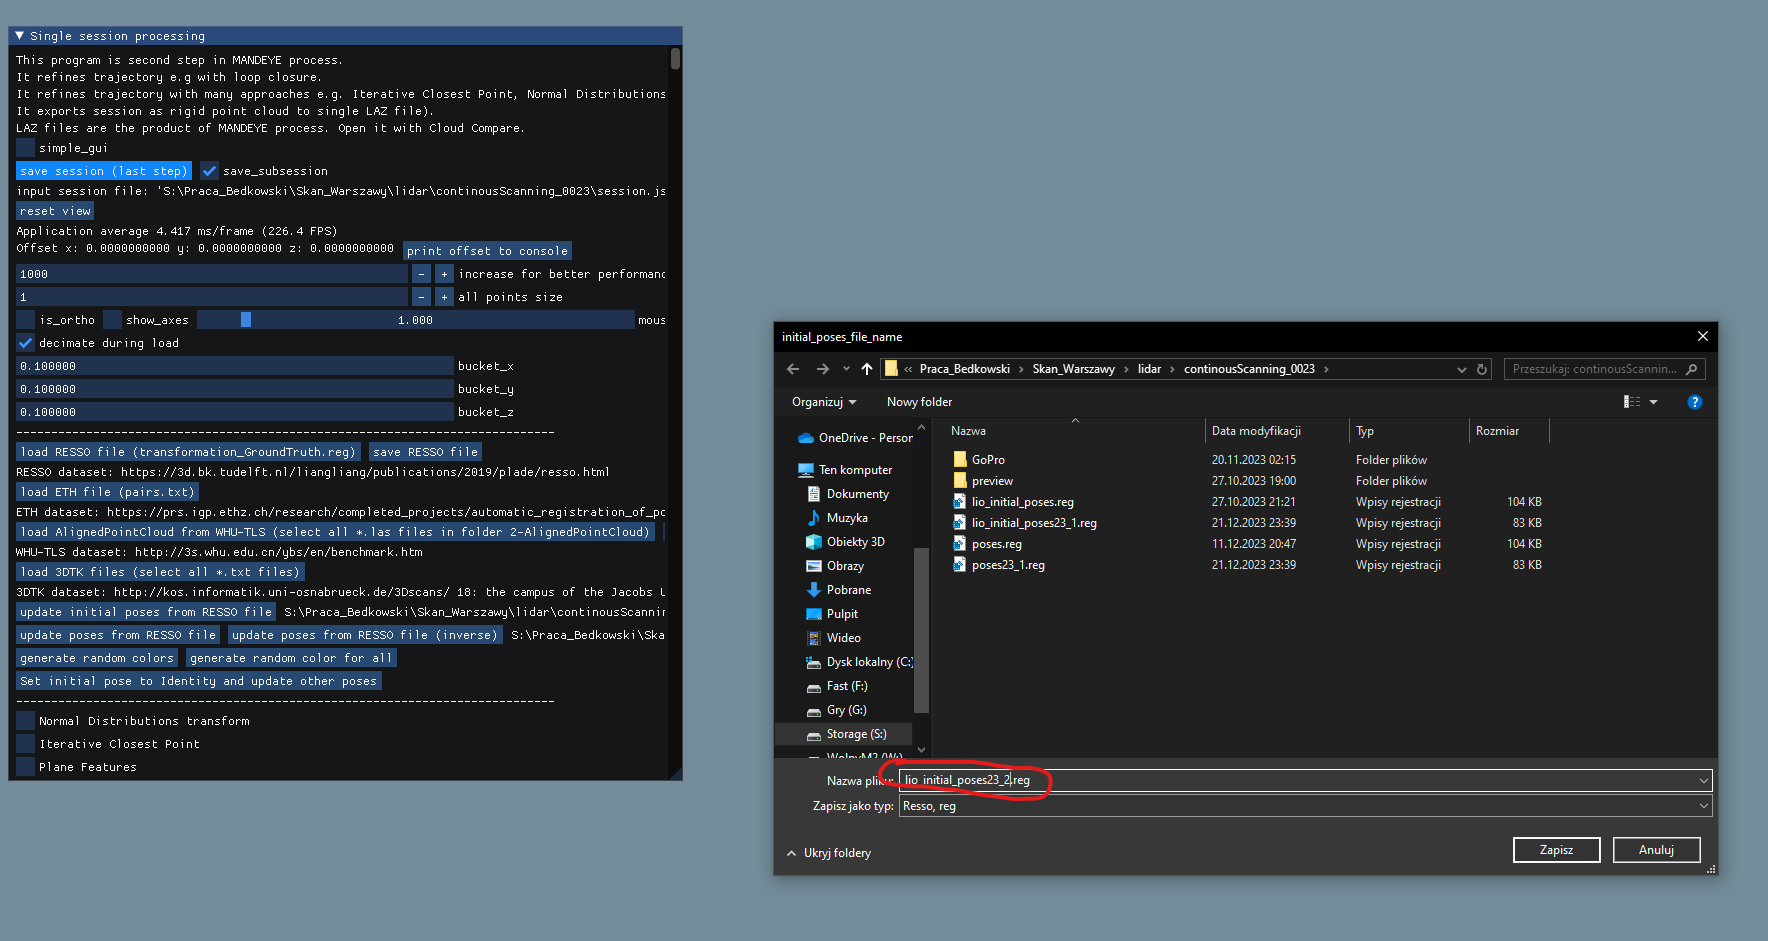
\includegraphics[width=\textwidth]{Cut_session6.png}
	\caption{Do the same as in previous step with initial poses file - create new file and save it.}
	\label{fig:25}
\end{figure}

\section{Step 3}
\begin{figure}[H]
	\centering
	\includegraphics[width=\textwidth]{20.png}
	\caption{Add sessions that you want to align.}
	\label{fig:26}
\end{figure}

\begin{figure}[H]
	\centering
	\includegraphics[width=\textwidth]{21.png}
	\caption{Choose session.json files - effects of the lidar odometry step.}
	\label{fig:27}
\end{figure}

\begin{figure}[H]
	\centering
	\includegraphics[width=\textwidth]{22.png}
	\caption{Click load sessions button and wait for the chosen sessions to load.}
	\label{fig:28}
\end{figure}

\begin{figure}[H]
	\centering
	\includegraphics[width=\textwidth]{23.png}
	\caption{When all of the sessions have loaded activate Manual Pose Graph Loop Closure Mode. If more than 2 sessions were loaded, deactivate sessions till two of them remain. After that the button should appear.}
	\label{fig:29}
\end{figure}

\begin{figure}[H]
	\centering
	\includegraphics[width=\textwidth]{24.png}
	\caption{Choose 2 individual scans of the same area, one from the first session, other from the second session and click add edge.}
	\label{fig:30}
\end{figure}

\begin{figure}[H]
	\centering
	\includegraphics[width=\textwidth]{25.png}
	\caption{Click manipulate active edge, then gizmo and as in \hyperref[fig:15]{the step 2} align scans as precisely as possible and then repeatedly use ICP till nothing changes.}
	\label{fig:31}
\end{figure}

\begin{figure}[H]
	\centering
	\includegraphics[width=\textwidth]{26.png}
	\caption{After aligning scans turn off Manual Pose Graph Loop Closure Mode, click Optimize and if everything is ok then click Save results. Should anything go wrong and sessions haven't orientated as planned just use Revert button. Repeat steps 3.13-3.15 until two sessions are aligned with a satisfying effect.}
	\label{fig:32}
\end{figure}

\begin{figure}[H]
	\centering
	\includegraphics[width=\textwidth]{27.png}
	\caption{At the end or in the middle of work you can save your project to .json file, which can be loaded next time multi session registration step 3 is used.}
	\label{fig:33}
\end{figure}
\pagebreak
\textbf{Last part describes the process of downloading, preparing and synchronizing ISOK ALS data (\url{http://www.gugik.gov.pl/projekty/isok/produkty}) with scans prepared through HDMapping software.}
Figures from \ref{fig:34} to \ref{fig:38} serve only as an example of how the process of gathering and preparing ALS data may look like.

To download ALS data Geoportal site will be used - \url{https://www.geoportal.gov.pl}.

\begin{figure}[H]
	\centering
	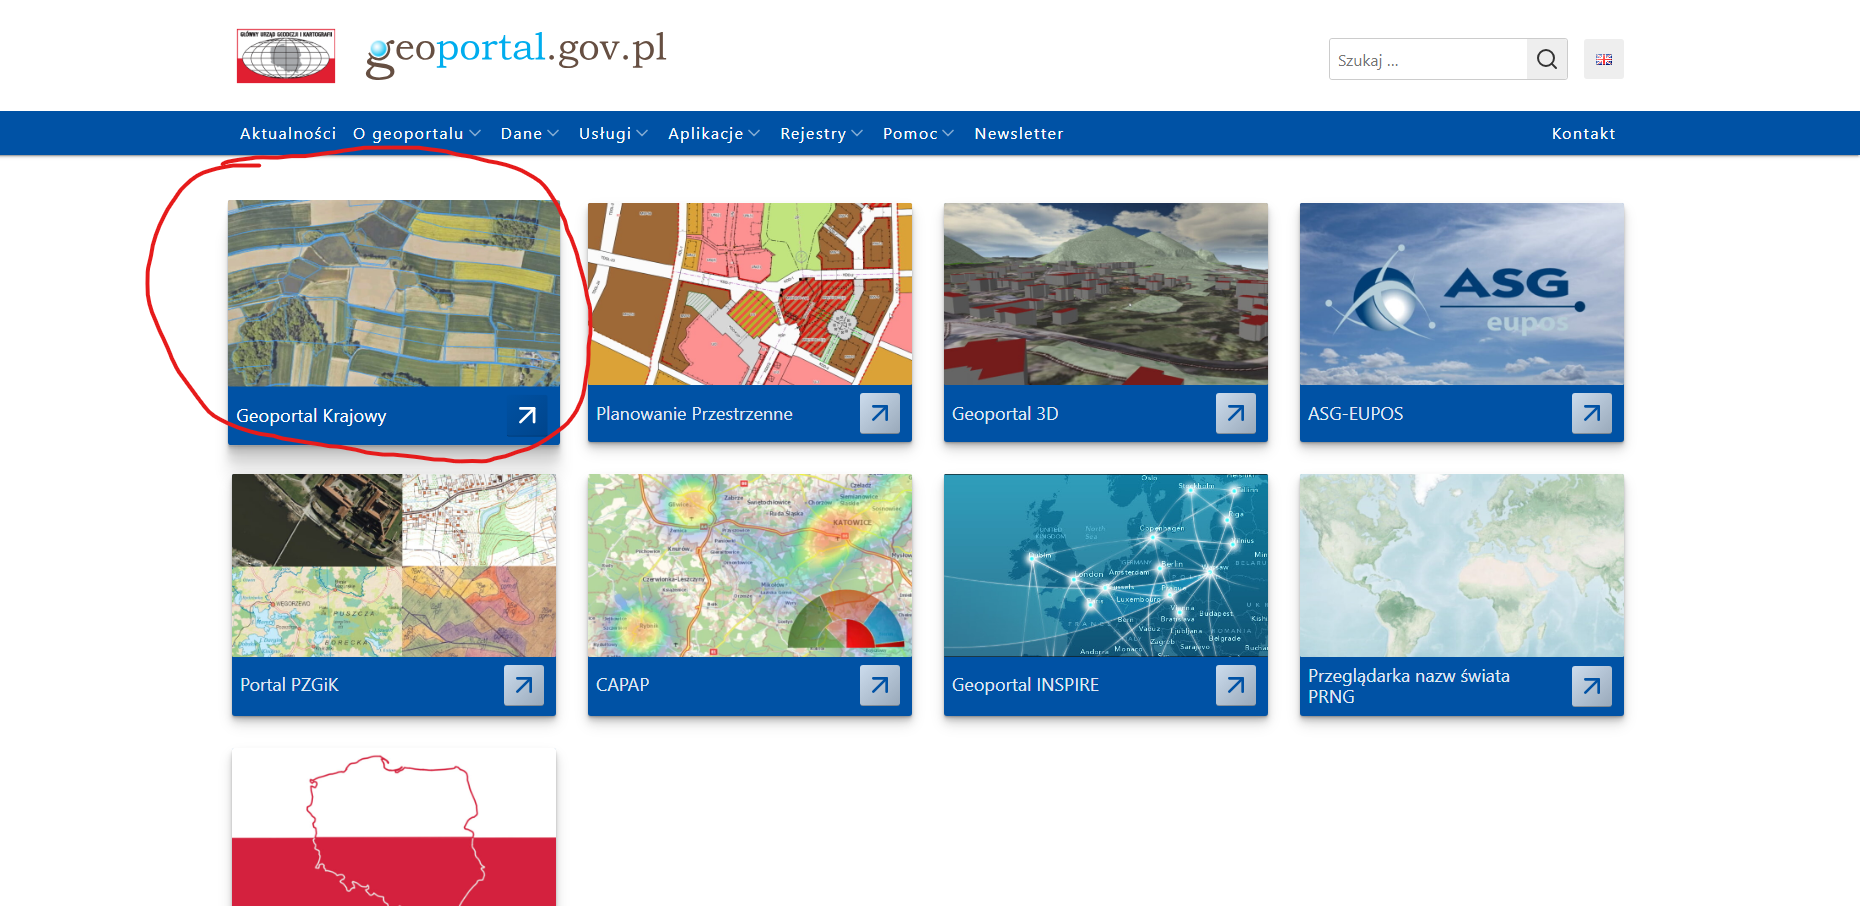
\includegraphics[width=\textwidth]{ISOK1.png}
	\caption{After \url{https://www.geoportal.gov.pl} site is loaded choose Geoportal krajowy tab.}
	\label{fig:34}
\end{figure}

\begin{figure}[H]
	\centering
	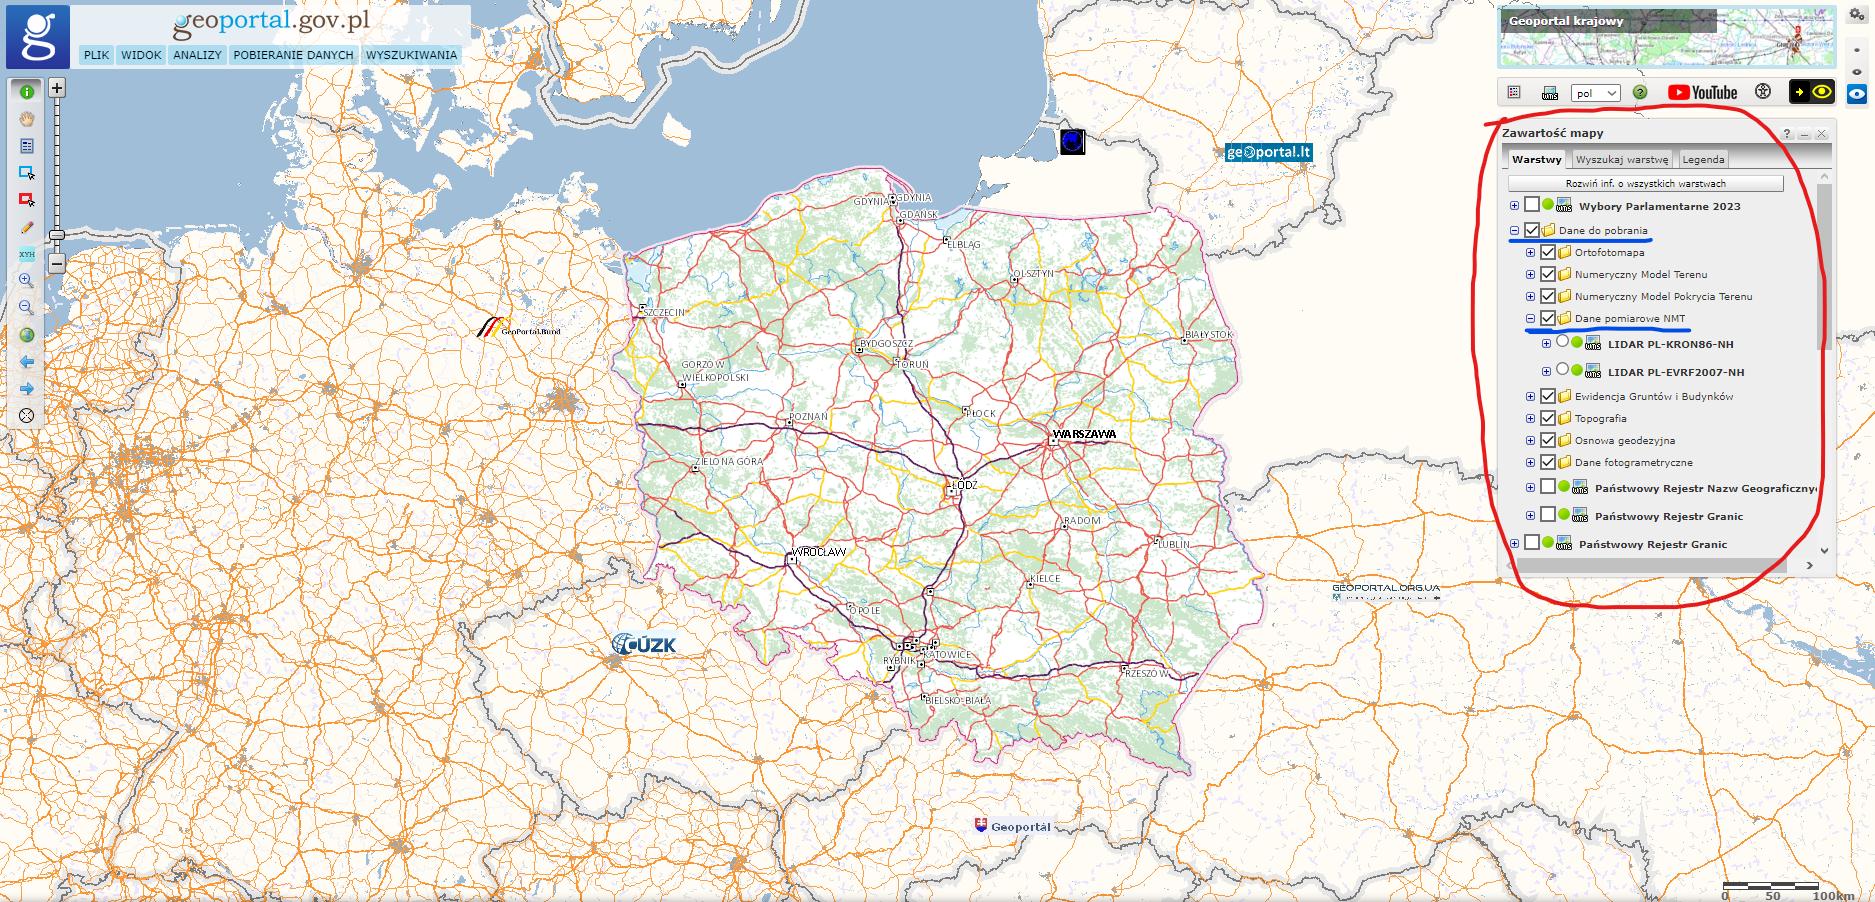
\includegraphics[width=\textwidth]{ISOK2.png}
	\caption{After Geoportal has loaded, on the right side of the screen select Dane do pobrania, then Dane pomiarowe NMT, where 2 options are possible.}
	\label{fig:35}
\end{figure}

\begin{figure}[H]
	\centering
	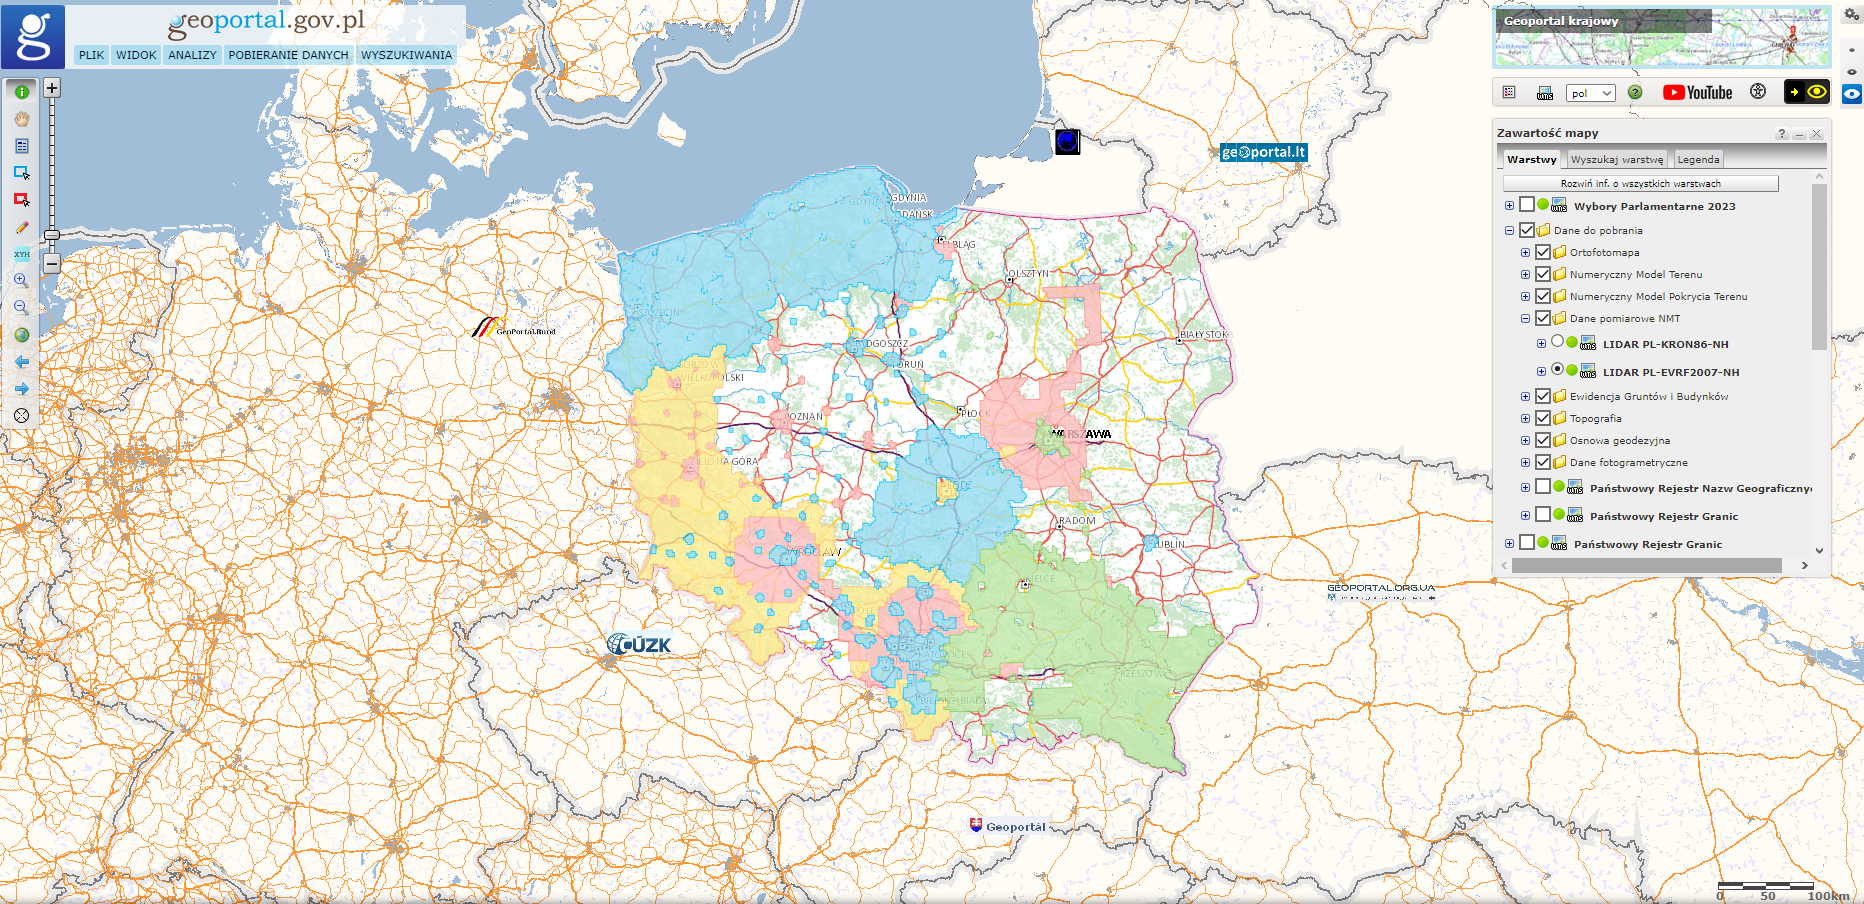
\includegraphics[width=\textwidth]{ISOK3.png}
	\caption{Whenever it is possible EVRF LIDAR version should be chosen over KRON36 version, as the former is more current than the latter. As can be seen on the screen there are parts without EVRF version and in such cases KRON86 is the only option.}
	\label{fig:36}
\end{figure}

\begin{figure}[H]
	\centering
	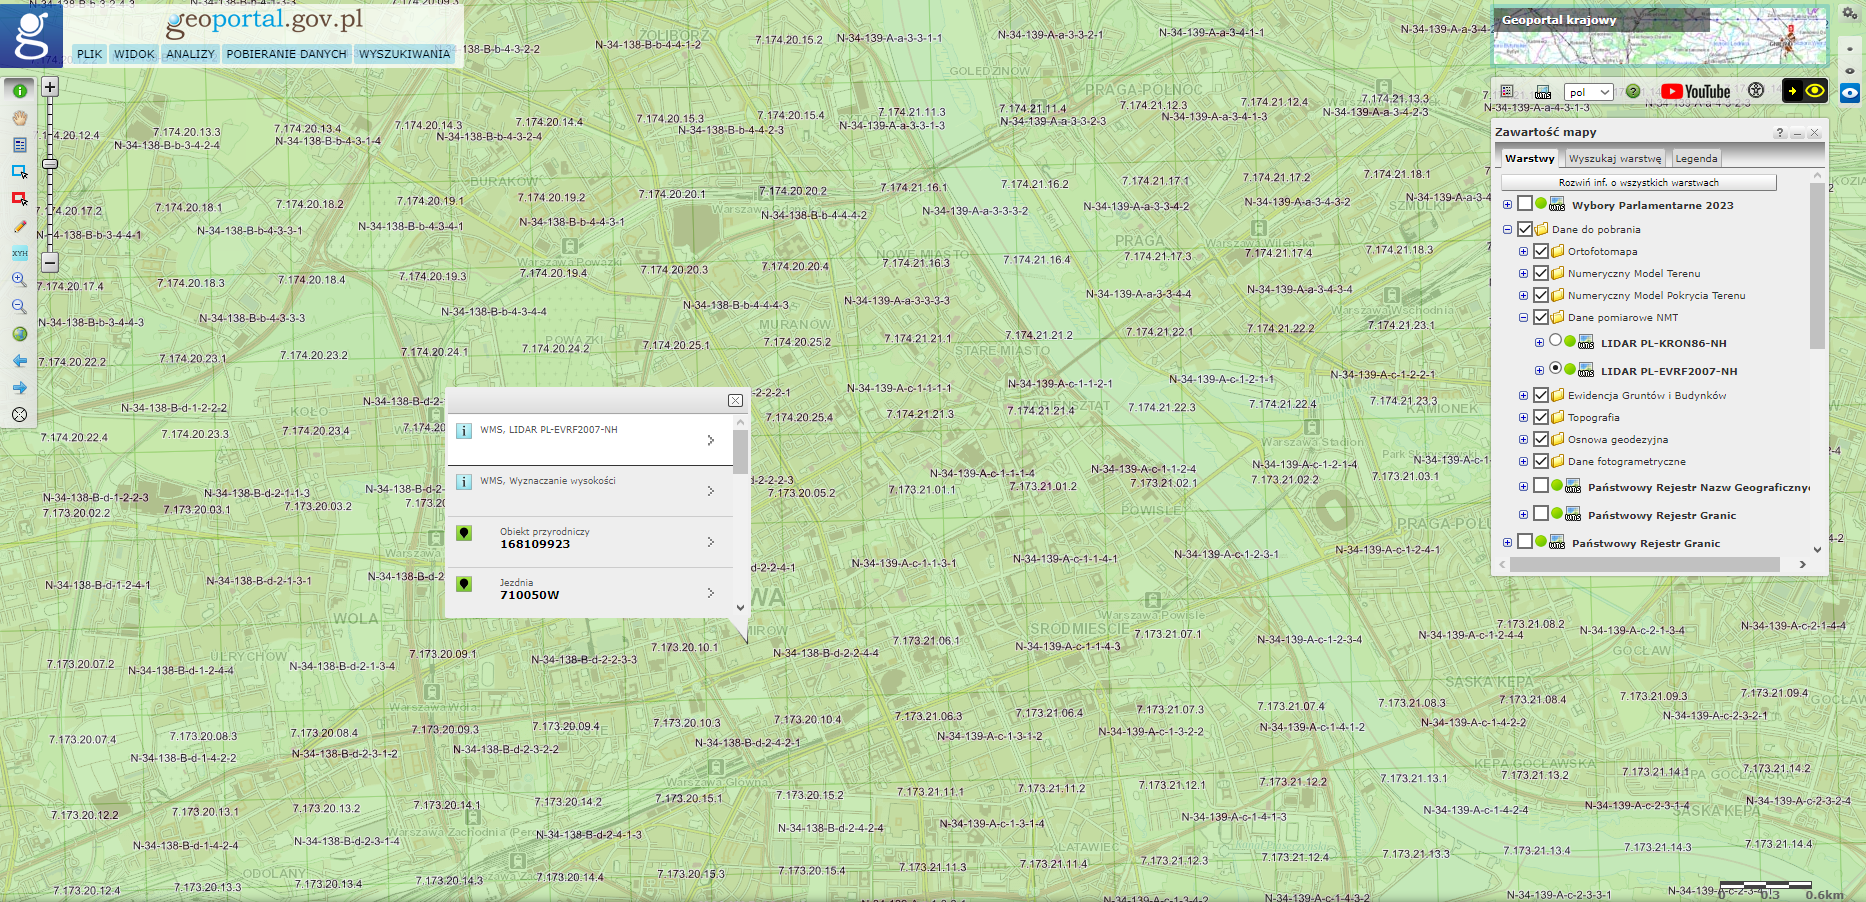
\includegraphics[width=\textwidth]{ISOK4.png}
	\caption{When LIDAR has been chosen zoom in to the map until tiles are seen. To download simply click on the tile with left mouse button and choose WMS, LIDAR.}
	\label{fig:37}
\end{figure}

\begin{figure}[H]
	\centering
	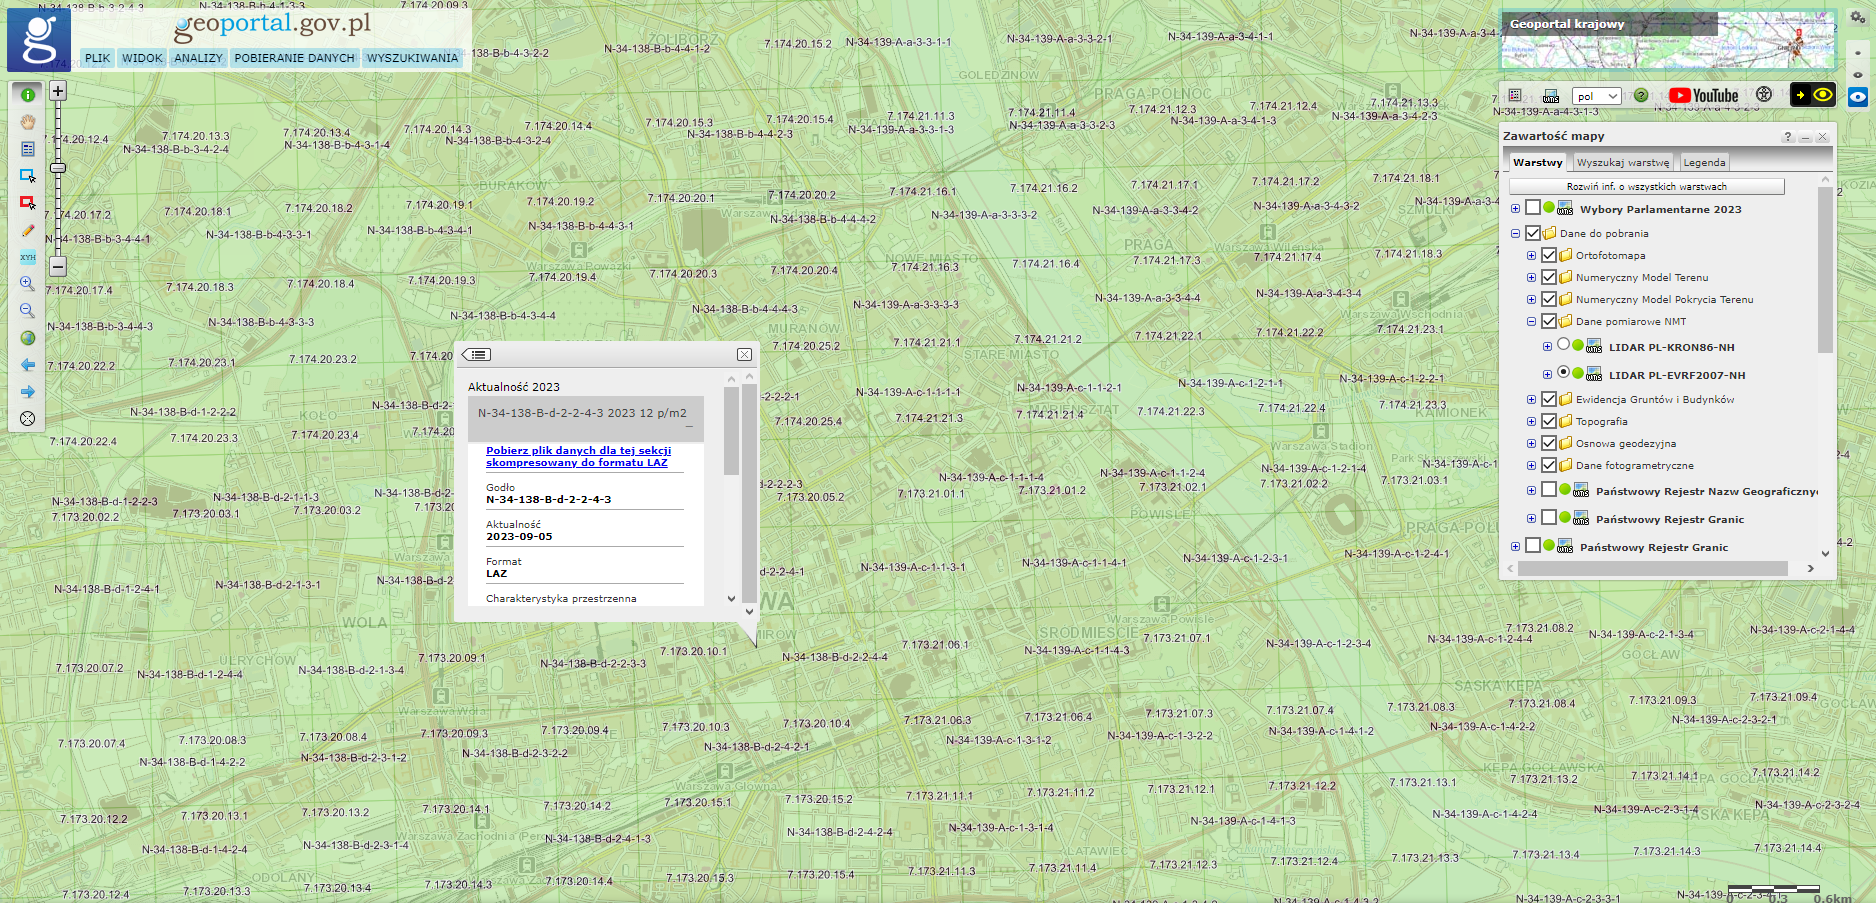
\includegraphics[width=\textwidth]{ISOK5.png}
	\caption{Then choose the newest version (usually the highest one) and use the link to download .laz file. Repeat this and previous step for every tile that covers your area of interest.}
	\label{fig:38}
\end{figure}

\begin{figure}[H]
	\centering
	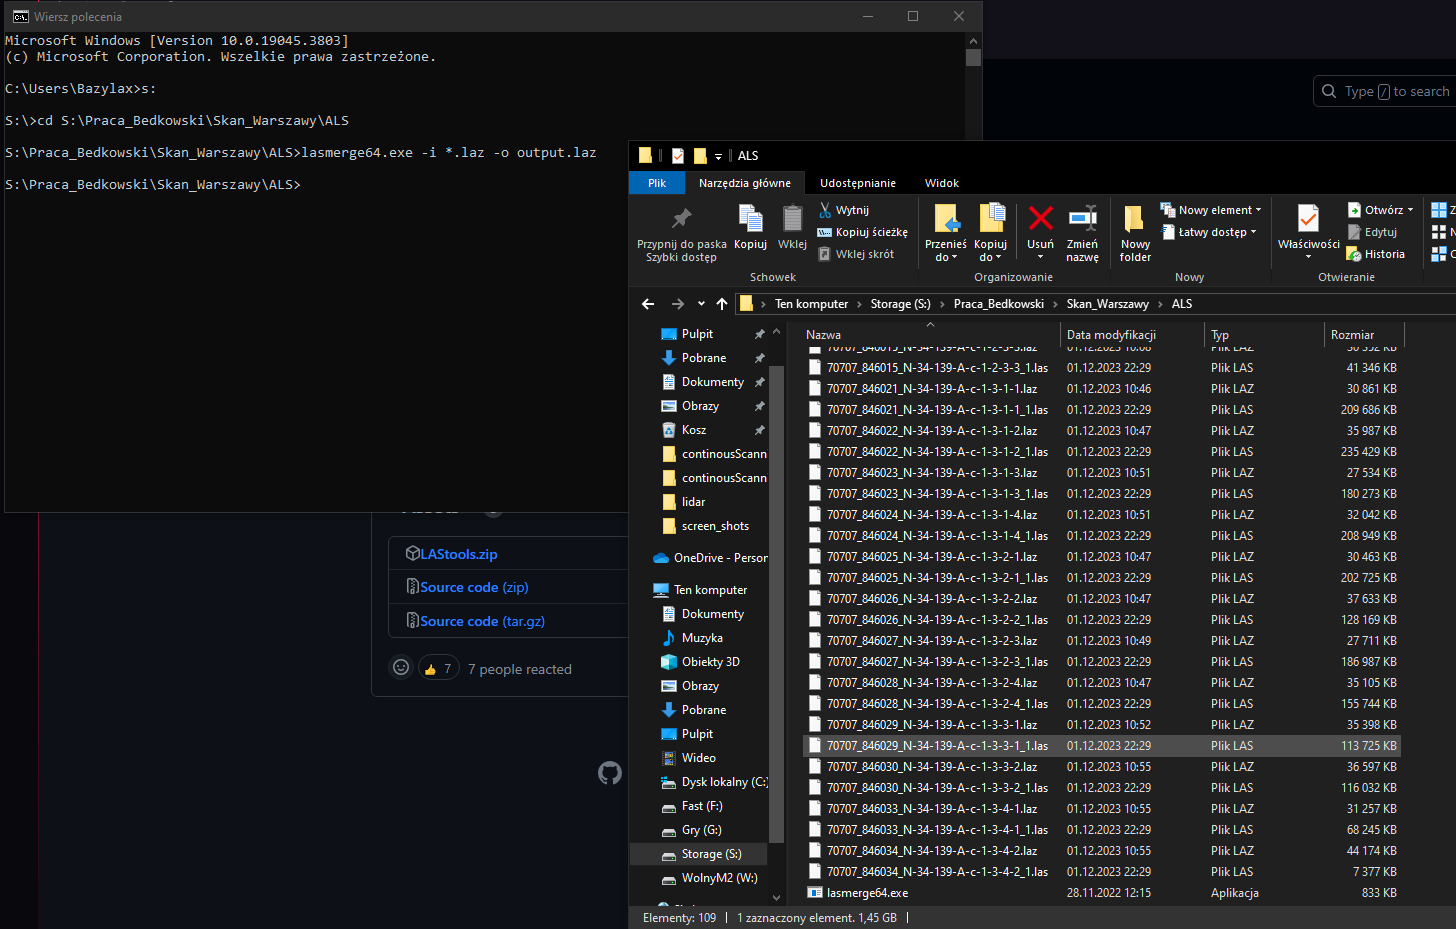
\includegraphics[width=\textwidth]{ISOK6.png}
	\caption{If merging downloaded tiles is needed, I recommend using LAStools software. Download LAStools.zip from release page (\url{https://github.com/LAStools/LAStools/releases/tag/v2.0.2}). From folder bin/ extract lasmerge64.exe and put it in the folder where tile .laz files are stored. Open windows command prompt, move to directory with .laz files and write command: 
	\textit{lasmerge64.exe -i *.laz -o <your output .laz file name>.laz}}
	\label{fig:39}
\end{figure}
